\chapter{Background and Related Work}

\section{Android Ecosystem}

\subsection{Android}

Android is a open souce mobile device operating system led by Google and
OHA (Open Handset Alliance). Android is a linux-based operating system with
several layers shown in Figure\ref{fig:android-system-architecture}.

\begin{figure}[!ht]
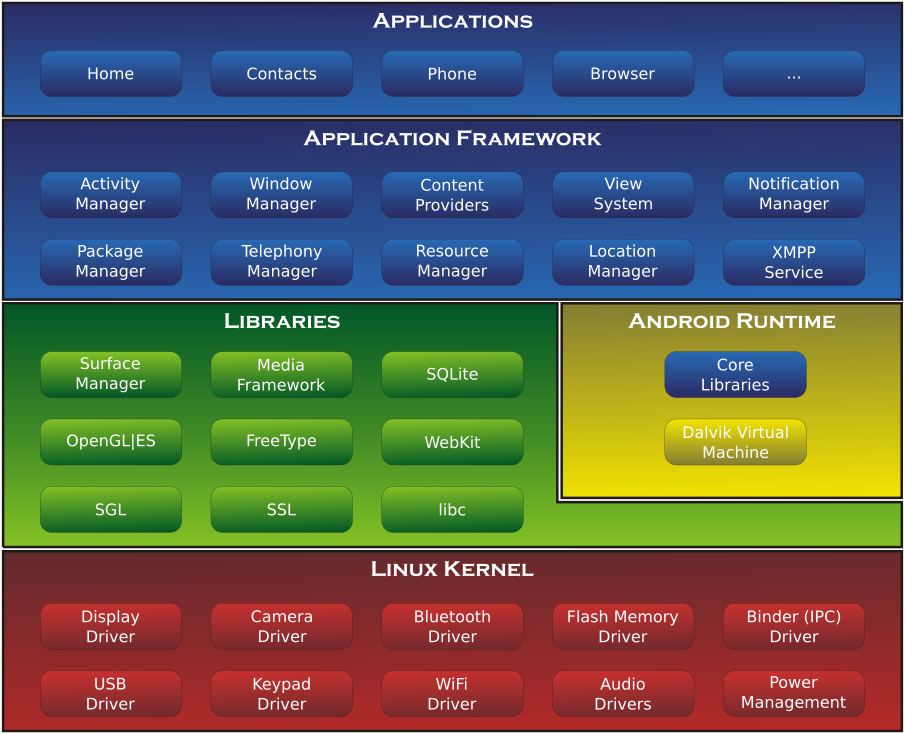
\includegraphics[width=0.8\textwidth]{img/Android-System-Architecture}
\caption{Android System Architecture}
\label{fig:android-system-architecture}
\end{figure}

\subsection{Android x86}

Android x86 is a project to port AOSP (Android Open Source Project) to x86
platform, and provides the ability to install Android on some x86 devices, such
as ASUS Eee PCs.

\subsection{Android Market}

Android market is a general term that desribes a online platform that provides
Android apps to install or download. Google Play is the largest and official
market.

\subsection{Android app and Dalvik VM}

Android apps are usually written in Java. To pack an app, the
source code (*.java) is first compile into Java bytecode (*.class). And then,
the Java bytecode will be compiled into Dalvik executable bytecode (*.dex)
along with native libraries. Finally, the Dalvik executable bytecode will be
compressed into zip format (*.apk).

To run an app, Android system will spawn a Dalvik VM to execute the Dalvik
executable bytecode. Each app is run by a Dalvik VM with a unique sysetm user
to prevent accessing each others data.

%\section{Symbolic Execution}
%\subsection{Symbolic Execution}
%\subsection{Concolic Execution}
%\subsection{Single Path Concolic Execution}
%
%\section{Common Vulnerabilities}
%\subsection{Stack Buffer Overflow}
%\subsection{Heap Overflow}
